% questions.tex —— 1981 年·全国卷（理科） · 题目内容片段（无答案）
% 由 tools/generate_projects.py 依来源总账自 1981/1981_数学真题_理_试题.md 生成，勿手改（改源 MD 后重跑）


\gkpart{理科数学}

\begin{gktip}
\textbf{来源说明}：本题面依据固定原卷 PDF《1981 理》第 1 页（印刷页码 17）逐题转录。源卷为单页题面，未附答案页；配套答案与解析由本库独立推导，\textbf{非官方标准答案}。正式题为第 1—9 题；卷末「附加题」栏一题在原卷中沿用大题号印作「10．」，本库作为附加题 10 保留在第 9 题之后，不计入正式题量。第 3 题为表格题，原表第三列供填答，此处照录为空白。第 7 题附所给对数表，按原卷三列照录。
\end{gktip}

\par\medskip

\begin{question}
\gkti{1}设 $A$ 表示有理数的集合，$B$ 表示无理数的集合，即设 $A=\{\text{\text{有理数}}\}$，$B=\{\text{\text{无理数}}\}$，试写出：

（1） $A\cup B$；

（2） $A\cap B$。

\end{question}
\begin{question}
\gkti{2}在 $A$、$B$、$C$、$D$ 四位候选人中，

（1） 如果选举正、副班长各一人，共有几种选法？写出所有可能的选举结果；

（2） 如果选举班委三人，共有几种选法？写出所有可能的选举结果。

\end{question}
\begin{question}
\gkti{3}下表所列各小题中，指出 $A$ 是 $B$ 的充分条件，还是必要条件，还是充要条件，或者都不是。

\begin{center}
\begin{tabular}{lll}
\toprule
$A$ & $B$ & $A$ 是 $B$ 的什么条件 \\
\midrule
四边形 $ABCD$ 为平行四边形 & 四边形 $ABCD$ 为矩形 &  \\
$a=3$ & $\lvert a\rvert=3$ &  \\
$\theta=150^\circ$ & $\sin\theta=\dfrac12$ &  \\
点 $(a,b)$ 在圆 $x^2+y^2=R^2$ 上 & $a^2+b^2=R^2$ &  \\
\bottomrule
\end{tabular}
\end{center}

\end{question}
\begin{question}
\gkti{4}写出余弦定理（只写一个公式即可），并加以证明。

\end{question}
\begin{question}
\gkti{5}解不等式（$x$ 为未知数）：

\nopagebreak[4]
\[
\begin{vmatrix}
x-a & b & -c\\
a & x-b & c\\
-a & b & x-c
\end{vmatrix}>0.
\]

\end{question}
\begin{question}
\gkti{6}用数学归纳法证明等式：

\nopagebreak[4]
\[
\cos\frac{x}{2}\cdot\cos\frac{x}{2^2}\cdot\cos\frac{x}{2^3}\cdot\cdots\cdot\cos\frac{x}{2^n}
=\frac{\sin x}{2^n\sin\frac{x}{2^n}}.
\]

对一切自然数 $n$ 都成立。

\end{question}
\begin{question}
\gkti{7}设 1980 年底我国人口以 10 亿计算。

（1） 如果我国人口每年比上年平均递增 $2\%$，那么到 2000 年底将达到多少？

（2） 要使 2000 年底我国人口不超过 12 亿，那么每年比上年平均递增率最高是多少？

下列对数值可供选用：

\begin{center}
\begin{tabular}{lll}
\toprule
 &  &  \\
\midrule
$\lg 1.0087=0.00377$ & $\lg 1.0092=0.00396$ & $\lg 1.0096=0.00417$ \\
$\lg 1.0200=0.00860$ & $\lg 1.2000=0.07918$ & $\lg 1.3098=0.11720$ \\
$\lg 1.4568=0.16340$ & $\lg 1.4859=0.17200$ & $\lg 1.5157=0.18060$ \\
\bottomrule
\end{tabular}
\end{center}

\end{question}
\begin{question}
\gkti{8}在 $120^\circ$ 的二面角 $P-a-Q$ 的两个面 $P$ 和 $Q$ 内，分别有点 $A$ 和点 $B$，已知点 $A$ 和点 $B$ 到棱 $a$ 的距离分别为 2 和 4，且线段 $AB=10$。

（1） 求直线 $AB$ 和棱 $a$ 所成的角；

（2） 求直线 $AB$ 和平面 $Q$ 所成的角。

\Needspace{0.4\textheight}
\end{question}
\begin{question}
\gkti{9}给定双曲线 $x^2-\dfrac{y^2}{2}=1$。

（1） 过点 $A(2,1)$ 的直线 $L$ 与所给的双曲线交于两点 $P_1$ 及 $P_2$，求线段 $P_1P_2$ 的中点 $P$ 的轨迹方程；

（2） 过点 $B(1,1)$ 能否作直线 $m$，使 $m$ 与所给双曲线交于两点 $Q_1$ 及 $Q_2$，且点 $B$ 是线段 $Q_1Q_2$ 的中点？这样的直线 $m$ 如果存在，求出它的方程；如果不存在，说明理由。

\Needspace{5\baselineskip}
\textbf{附加题 10．} 已知以 $AB$ 为直径的半圆有一个内接正方形 $CDEF$，其边长为 1（如图）。设 $AC=a$，$BC=b$，作数列

\nopagebreak[4]
\[
u_1=a-b,\quad u_2=a^2-ab+b^2,\quad u_3=a^3-a^2b+ab^2-b^3,\quad\cdots,\quad
u_k=a^k-a^{k-1}b+a^{k-2}b^2-\cdots+(-1)^k b^k;
\]

求证：$u_n=u_{n-1}+u_{n-2}$（$n\geqslant 3$）。
\nopagebreak[4]
\begin{center}% 1981 年全国卷（理科）第 10 题：以 AB 为直径的半圆及其内接正方形 CDEF（按源卷布局）。
% 圆心 O 为原点、半径 sqrt(5)/2；F、C 关于 O 对称，边长为 1，E、D 在半圆上。
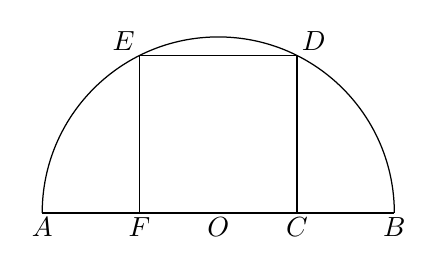
\begin{tikzpicture}[scale=2.0, line width=0.45pt,
  every node/.style={inner sep=1.5pt}]
  \pgfmathsetmacro{\R}{sqrt(5)/2}
  \coordinate (O) at (0,0);
  \coordinate (A) at (-\R,0);
  \coordinate (B) at (\R,0);
  \coordinate (F) at (-0.5,0);
  \coordinate (C) at (0.5,0);
  \coordinate (E) at (-0.5,1);
  \coordinate (D) at (0.5,1);
  % 半圆与直径 AB
  \draw (A) arc (180:0:\R);
  \draw (A) -- (B);
  % 内接正方形 CDEF
  \draw (F) -- (E) -- (D) -- (C) -- cycle;
  \node[anchor=north] at (A) {$A$};
  \node[anchor=north] at (F) {$F$};
  \node[anchor=north] at (O) {$O$};
  \node[anchor=north] at (C) {$C$};
  \node[anchor=north] at (B) {$B$};
  \node[anchor=south east] at (E) {$E$};
  \node[anchor=south west] at (D) {$D$};
\end{tikzpicture}
\end{center}
\nopagebreak[4]

\end{question}